\documentclass[usenames,dvipsnames,8pt,aspectratio=169]{beamer}
\usepackage{amsmath,amsfonts,amssymb}
\usepackage{mathtools}
\usepackage{etex} %for Windows
\usepackage[utf8]{inputenc}
\usepackage[english, russian]{babel} 

%\usepackage{microtype}			% Better interword spacing and additional kerning.
\usepackage{ellipsis}			% Adjusted space with \dots between two words.
\usepackage{graphicx}
\usepackage{pstricks}

\usepackage{xcolor}


\usepackage{changepage}

\usepackage{algorithm}
\usepackage{algpseudocode}
%\usepackage[]{algorithm2e}
%\usepackage{algorithmic}

%\usepackage{tcolorbox}

\addtobeamertemplate{footline}{%
	\setlength\unitlength{1ex}%
	\begin{picture}(0,0) 
	% \put{} defines the position of the frame
	\put(155,0){\makebox(0,0)[bl]{
			%
\includegraphics[scale=0.65]{white_square}
			%
\includegraphics[scale=0.65]{dark_square}
			
\includegraphics[scale=0.65]{grey_circle}
	}}%
	\end{picture}%
}{}

\usepackage{tikz}
\usetikzlibrary{tikzmark,calc}
\usetikzlibrary{positioning, backgrounds}
\usetikzlibrary{arrows, chains, matrix, scopes, patterns, shapes, fit}
\usetikzlibrary{mindmap,trees,shadows}
\usetikzlibrary{decorations.pathreplacing}

\usepackage{pgfplots}

\pgfmathdeclarefunction{gauss}{2}{%
	\pgfmathparse{1/(#2*sqrt(2*pi))*exp(-((x-#1)^2)/(2*#2^2))}%
}


\tikzset{
	invisible/.style={opacity=0},
	visible on/.style={alt={#1{}{invisible}}},
	alt/.code args={<#1>#2#3}{%
		\alt<#1>{\pgfkeysalso{#2}}{\pgfkeysalso{#3}} % \pgfkeysalso doesn't change the path
	},
}

\newcommand\strikeout[2][]{%
	\begin{tabular}[b]{@{}c@{}} 
		\makebox(0,0)[cb]{{#1}} \\[-0.2\normalbaselineskip]
		\rlap{\color{Orange}\rule[0.5ex]{\widthof{#2}}{1.5pt}}#2
\end{tabular}}

\newcommand\Fontvi{\fontsize{11}{13.2}\selectfont}

\usepackage{listings} % for C++ code

\usepackage{braket}
%\usepackage[braket, qm]{qcircuit}



\usepackage[T1]{fontenc}
%\usepackage[sfdefault,scaled=.85]{FiraSans}
%\usepackage{newtxsf}
%\usepackage[nomap]{FiraMono}





\usefonttheme[onlymath]{serif}
\renewcommand\sfdefault{cmbr}

\renewcommand{\bfdefault}{sb}

\definecolor{CharCoalDark}{RGB}{13, 16, 19}
\definecolor{Orange}{RGB}{255, 165,0}
\definecolor{DarkOrange}{RGB}{255, 165,0}
\definecolor{LightSalmon}{RGB}{255, 160, 122}
\definecolor{LeafGreen}{RGB}{34, 139,  34}
\definecolor{Coral}{RGB}{255, 127, 80}
\definecolor{DarkTurquoise}{RGB}{0, 206, 209}

\definecolor{darkslateblue}{RGB}{72,61,139}

%\newtheorem{defRus}{Определение}
%\newtheorem{thmRus}{Теорема}
%s\newtheorem{corRus}{Следствие}

\def\darktheme{}
\ifdefined\darktheme
	\setbeamercolor{background canvas}{bg=CharCoalDark}
	\setbeamerfont{title}{series=\bfseries}
	\setbeamercolor{title}{fg=Orange}
	\setbeamercolor{section in toc}{fg=white}
	\setbeamercolor{frametitle}{fg=Orange}
	\setbeamercolor{normal text}{fg=white}
	%\setbeamercolor{normal text}{fontsize=12pt}
	\setbeamercolor{itemize item}{fg=Orange}
	\setbeamercolor{itemize item item}{fg=Orange}
	\setbeamercolor{enumerate item}{fg=Orange}
	\setbeamercolor{block title}{bg=DarkOrange,fg=white}
	\setbeamerfont{block title}{series=\bfseries}
	
	\setbeamertemplate{itemize item}[circle]
	%\setbeamertemplate{itemize subitem}[$\checkmark$]
	\setbeamertemplate{itemize subitem}{\color{Orange}\Large$\textbullet$}
	\setbeamertemplate{itemize subitem}{\color{Orange} \tiny $\blacksquare$}
\else
	\setbeamercolor{background canvas}{bg=white}
	\setbeamerfont{title}{series=\bfseries}
	\setbeamercolor{title}{fg=darkslateblue}
	\setbeamercolor{section in toc}{fg=black}
	\setbeamercolor{frametitle}{fg=darkslateblue}
	\setbeamercolor{normal text}{fg=black}
	%\setbeamercolor{normal text}{fontsize=9pt}
	\setbeamercolor{itemize item}{fg=darkslateblue}
	\setbeamercolor{itemize item item}{fg=darkslateblue}
	\setbeamercolor{enumerate item}{fg=darkslateblue}
	\setbeamercolor{block title}{bg=darkslateblue,fg=white}
	\setbeamerfont{block title}{series=\bfseries}
	
	\setbeamertemplate{itemize item}[circle]
	%\setbeamertemplate{itemize subitem}[$\checkmark$]
	\setbeamertemplate{itemize subitem}{\color{blue}\Large$\textbullet$}
	\setbeamertemplate{itemize subitem}{\color{blue} \tiny $\blacksquare$}

\fi

% footnote without a marker
\newcommand\blfootnote[1]{%
	\begingroup
	\renewcommand\footnoterule{}
	\renewcommand\thefootnote{}\footnote{#1}%
	\addtocounter{footnote}{-1}%
	\endgroup
}

\newcommand*{\Scale}[2][4]{\scalebox{#1}{\ensuremath{#2}}}%

\newcommand\Item[1][]{%
	\ifx\relax#1\relax  \item \else \item[#1] \fi
	\abovedisplayskip=0pt\abovedisplayshortskip=0pt~\vspace*{-\baselineskip}}

\pgfdeclareradialshading{ring}{\pgfpoint{0cm}{0cm}}%
{rgb(0cm)=(1,1,1);
	rgb(0.7cm)=(1,1,1);
	rgb(0.719cm)=(1,1,1);
	rgb(0.72cm)=(0.975,0,0);
	rgb(0.9cm)=(1,1,1)}

\usepackage[absolute,overlay]{textpos} %to clip to a corner
\newcommand\FrameText[1]{%
	\begin{textblock*}{\paperwidth}(\textwidth-35pt, 10 pt)
		\raggedright #1\hspace{.5em}
\end{textblock*}}

\newcommand\myeq{\stackrel{\mathclap{\normalfont\mbox{?}}}{=}}


\makeatletter
\let\save@measuring@true\measuring@true
\def\measuring@true{%
	\save@measuring@true
	\def\beamer@sortzero##1{\beamer@ifnextcharospec{\beamer@sortzeroread{##1}}{}}%
	\def\beamer@sortzeroread##1<##2>{}%
	\def\beamer@finalnospec{}%
}
\makeatother

\AtBeginSection[]
{
	\begin{frame}<beamer>
		\frametitle{Outline}
		\tableofcontents[currentsection]
	\end{frame}
}


%\institute{ENS Lyon}
\author{\\ [10pt]
}
\titlegraphic{
	
	%\includegraphics[width=2.5cm]{erc_logo_gray}\hspace*{2.5cm}~%
	%\includegraphics[width=4.0cm]{ens_logo_gray}
}
\title{Лекция №2 \\[10pt]
		Часть 2. Потоковый шифр}

\date{ Елена Киршанова \\  \textbf{Курс ``Основы криптографии''} \\  }


\setbeamertemplate{navigation symbols}{} %removes navigation

% proper highlightling of a code-snippet
\lstset{language=C++,
	keywordstyle=\color{magenta},
	stringstyle=\color{Goldenrod},
	commentstyle=\color{gray},
	breaklines=false,
	%morecomment=[l][\color{magenta}]{\#}
}

%\setlength{\parskip}{8pt}
% ==================================================================
% Definitions for this paper
% ==================================================================
\mathchardef\hyphen="2D

\usepackage{multirow}
\usepackage{multicol} % For multiple coloumn environments
%\usepackage{stmaryrd} % For set brackets
% \setlength{\columnsep}{15pt} % Defining the coloumn seperation
% \setlength{\columnseprule}{1pt} % Place a line between coloumns
% \newcommand{\tab}{\hspace*{2em}}

%subscripts

\newcommand*\SmallTextScript[2]{{\mathchoice{\displaystyle #2}
		{\textstyle #2}%dito
		{\scalebox{#1}{\ensuremath{\scriptstyle #2}}}%
		{\scalebox{#1}{\ensuremath{\scriptscriptstyle #2}}}%
}}


% ADVERSARIES AND SUCH
\newcommand*{\poly}{\ensuremath{\mathrm{poly}}}
\newcommand*{\eps}{\ensuremath{\varepsilon}}
\newcommand*{\alg}{\ensuremath{\mathcal{A}}}

% GROUPS/DISTRIBUTIONS/SETS/LISTS
\newcommand{\N}{{{\mathbb N}}}
\newcommand{\Z}{{{\mathbb Z}}}
\newcommand*{\IZ}{\ensuremath{\mathbb{Z}}}
\newcommand*{\IN}{\ensuremath{\mathbb{N}}}
\newcommand*{\IQ}{\ensuremath{\mathbb{Q}}}
\newcommand{\R}{{{\mathbb R}}}
\newcommand*{\IR}{{{\mathbb R}}}
\newcommand{\Zp}{\ints_p} % Integers modulo p
\newcommand{\Zq}{\ints_q} % Integers modulo q
\newcommand{\Zn}{\ints_N} % Integers modulo N
\newcommand{\F}{\ensuremath{\mathbb{F}}}
\newcommand{\CC}{\ensuremath{\mathbb{C}}}

\newcommand{\GF}{\ensuremath{\mathbb{F}_2}}
\newcommand{\GFn}{\ensuremath{\mathbb{F}^n_2}}

%%% ALGORITHMS/PROCEDURES %%%
\newcommand{\Dec}{\textsf{Dec}}
\newcommand{\Enc}{\textsf{Enc}}
\newcommand{\KeyGen}{\textsf{KeyGen}}
\newcommand{\Gen}{\textsf{Gen}}
\newcommand{\sk}{\textsf{sk}}
\newcommand{\pk}{\textsf{pk}}
\newcommand{\vk}{\textsf{vk}}
\newcommand{\mesS}{\ensuremath{\mathcal{M}}}
\newcommand{\keyS}{\ensuremath{\mathcal{K}}}
\newcommand{\cipS}{\ensuremath{\mathcal{C}}}
\newcommand{\tagS}{\ensuremath{\mathcal{T}}}
\newcommand{\mactag}{\textsf{tag}}
\newcommand{\Hash}{\ensuremath{\mathcal{H}}}
\newcommand{\EID}{\ensuremath{\mathtt{EphID}}}


\newcommand{\adv}{\ensuremath{\mathcal{A}}}

\newcommand{\LWE}{\mathsf{LWE}}
\newcommand{\DCP}{\mathsf{DCP}}
\newcommand{\EDCP}{\mathsf{EDCP}}
\newcommand{\UEDCP}{\mathsf{U \text{-} EDCP}}
\newcommand{\GEDCP}{\mathsf{G \text{-} EDCP}}



%% Landau and proba
\newcommand{\bigO}{\mathcal{O}}
\newcommand*{\OLandau}{\bigO}
\newcommand*{\WLandau}{\Omega}
\newcommand*{\xOLandau}{\widetilde{\OLandau}}
\newcommand*{\xWLandau}{\widetilde{\WLandau}}
\newcommand*{\TLandau}{\Theta}
\newcommand*{\xTLandau}{\widetilde{\TLandau}}
\newcommand{\smallo}{o} %technically, an omicron
\newcommand{\wLandau}{\omega}
\newcommand{\negl}{\mathrm{negl}}
\newcommand*\PROB\Pr 
\DeclareMathOperator*{\EXPECT}{\mathbb{E}}
\DeclareMathOperator*{\VARIANCE}{\mathbb{V}}
\DeclareMathOperator*{\LOGBIAS}{\mathbb{LB}}

\newcommand{\supp}{\ensuremath{\mathsf{sup}}}
\newcommand{\Distr}{\ensuremath{\mathcal{D}}}

% Lattices

% \newcommand{\coset}{\Lambda} % Lambda Lattice
% \newcommand{\cosetPerp}{\Lambda^{\bot}} % Lambda_Perp Lattice
% \newcommand{\gadget}{\textbf{G}} %Gaget matrix
% \newcommand{\mes}{\textbf{m}} %message vector
% \newcommand{\AMat}{\textbf{A}} %A matrices
% \newcommand{\BMat}{\textbf{B}} %B matrices
% \newcommand{\RMat}{\textbf{R}} %R matrices
% \newcommand{\HMat}{\textbf{H}} %H matrices
% \newcommand{\XMat}{\textbf{X}} %H matrices
% \newcommand{\mbar}{\bar{m}} %mBar dimension
% % \newcommand{\gauss}{\mathcal{D}} % gaussian distribution
% \newcommand{\Id}{\textbf{I}} % Identity matrix
% \newcommand{\er}{\textbf{e}} % gaussian distr. vectors
% % \newcommand{\cipher}{\textit{c}} % ciphertext
% \newcommand{\Olwe}{\mathcal{O}_{\textsf{LWE}}} %LWE oracle
% \newcommand{\OSample}{\mathcal{O}_{Sample}} %LWE oracle
% \newcommand{\SigmaB}{\boldsymbol{\Sigma}} %semi-deifinite matrix Sigma%
% % \newcommand{\mods}{\text{ mod}}


%Vectors and Matrices

\newcommand{\AMat}{\mathbf{A}} %A matrices
\newcommand{\BMat}{\mathbf{B}} %B matrices
\newcommand{\DMat}{\mathbf{D}} %Diagonal


\newcommand{\HMat}{\ensuremath{\mathbf{H}}}
\newcommand{\QMat}{\ensuremath{\mathbf{Q}}}
\newcommand{\Id}{\ensuremath{\mathbf{I}}}
\newcommand{\ZeroM}{\textbf{0}} % Zero matrix

\newcommand{\avec}{\ensuremath{\mathbf{a}}}
\newcommand{\bvec}{\ensuremath{\mathbf{b}}}
\newcommand{\cvec}{\ensuremath{\mathbf{c}}}
\newcommand{\evec}{\ensuremath{\mathbf{e}}}
\newcommand{\rvec}{\ensuremath{\mathbf{r}}}
\newcommand{\svec}{\ensuremath{\mathbf{s}}}
\newcommand{\tvec}{\ensuremath{\mathbf{t}}}
\newcommand{\vvec}{\ensuremath{\mathbf{v}}}
\newcommand{\zvec}{\ensuremath{\mathbf{z}}}
\newcommand{\xvec}{\ensuremath{\mathbf{x}}}
\newcommand{\yvec}{\ensuremath{\mathbf{y}}}
\newcommand{\uvec}{\ensuremath{\mathbf{u}}}
\newcommand{\zerovec}{\ensuremath{\mathbf{0}}}

\newcommand{\nth}{^{\mathrm{th}}}
\newcommand{\nd}{^{\mathrm{nd}}}

\newcommand{\RepMMT}{\ensuremath{\mathcal{R}_{\protect\SmallTextScript{0.70}{\texttt{MMT}}}}}
\newcommand{\RepBJMM}{\ensuremath{\mathcal{R}_{\protect\SmallTextScript{0.70}{\texttt{BJMM}}}}}
\newcommand{\XOR}{\ensuremath{\mathtt{3XOR}}}


% % % % % \newcommand{\mb}[1]{\mathbf{#1}} % does not compile otherwise
%%% Removed by Gotti; this is just asking to screw up with packages that (properly) define \mb (mathbold)

% \newcommand{\bL}{\|\bvec_1\|} % b1 length that appears way too often
% \newcommand{\dL}{\|\dvec_1\|} % b1 length that appears way too oftend

%Norms and Scalar products

\newcommand*\abs[1]{\left\lvert#1\right\rvert}
\newcommand*\norm[1]{\left\lVert#1\right\rVert}
\newcommand*\normalabs[1]{\lvert#1\rvert} 
\newcommand*\normalnorm[1]{\lVert#1\rVert}
\newcommand*\bignorm[1]{\bigl\lVert#1\bigr\rVert}
\newcommand*\bigabs[1]{\bigl\lvert#1\bigr\rvert}
\newcommand*\Bigabs[1]{\Bigl\lvert#1\Bigr\rvert}
\newcommand*{\ScProd}[2]{\ensuremath{\langle#1\mathbin{,}#2\rangle}} %Scalar Product
% \newcommand*{\ScProd}[2]{\ensuremath{\langle#1 \:{,}\:#2\rangle}} %Scalar Product
\newcommand*{\bigScProd}[2]{\ensuremath{\bigl\langle#1\mathbin{,}#2\bigr\rangle}} %Scalar Product
\newcommand*{\BigScProd}[2]{\ensuremath{\Bigl\langle#1\mathbin{,}#2\Bigr\rangle}} %Scalar Product
\newcommand{\dist}{\ensuremath{\text{dist}}}


%Some other math operators

\DeclareMathOperator{\Span}{Span} %span of vectors
\DeclareMathOperator{\vol}{\mathrm{vol}} %volume
\DeclareMathOperator{\LW}{LambertW} %Lambert W function
\DeclareMathOperator{\SD}{SD}
\DeclareMathOperator{\gradient}{grad}
\DeclareMathOperator{\TRACE}{Tr}
\newcommand*{\dDR}{\mathrm{d}} %de-Rham-Differential (the d in dx, dy, dz and so on)


%Lists
\renewcommand{\L}{\ensuremath{\mathcal{L}}}

\renewcommand{\P}{\ensuremath{\mathcal{P}}}

\newcommand*{\Lout}{\ensuremath{\L_{\mkern-0.5mu\protect\SmallTextScript{0.85}{\textup{out}}}}}
\newcommand*{\Sout}{\ensuremath{S_{\mkern-0.5mu\protect\SmallTextScript{0.85}{\textup{out}}}}}
\newcommand{\wt}{\ensuremath{\mathit{wt}}}


\newcommand*{\softO}{\widetilde{\bigO}}

\newcommand{\const}{\mathsf{c}} 


\newcommand{\transpose}{\mkern0.7mu^{\mathsf{ t}}}

%proper overline reduced by 1.5mu
\newcommand{\overbar}[1]{\mkern 1.5mu\overline{\mkern-1.5mu#1\mkern-1.5mu}\mkern 1.5mu}

\DeclareMathOperator{\erf}{erf} %error function
\DeclareMathOperator{\erfc}{erfc} %complementary error function
\newcommand{\Er}{\ensuremath{\mathrm{Er}}} %complementary error function


% LATTICES

\newcommand{\Lat}{\ensuremath{\mathcal{L}}}
\newcommand*{\Sphere}[1]{\ensuremath{\mathsf{S}^{#1}}}
%\DeclareMathOperator{\Conf}{Conf}
\newcommand{\Conf}{\mathcal{C}}

%Thick line for table
\setlength{\doublerulesep}{0pt}
\newcommand{\thickline}{\hline\hline\hline}


%circled text
\newcommand*\circled[1]{\tikz[baseline=(char.base)]{
    \node[shape=circle,draw,inner sep=0.3 pt] (char) {\scriptsize #1};}}


%Fix Algorithmicx package
\def\NoNumber#1{{\def\alglinenumber##1{}\State #1}\addtocounter{ALG@line}{-1}}

%For comments
\newcommand{\GColor}{ForestGreen}  %Damiens' color
\newcommand{\EColor}{MidnightBlue} %Elena's color

\newcommand*{\E}[1]{{\color{\EColor} #1} } 
\newcommand*{\G}[1]{{\color{\GColor} #1} } 

%Proper limit with the subscript underneath
% \newcommand{\Lim}[1]{\raisebox{0.5ex}{\scalebox{0.8}{$\displaystyle \lim_{#1}\;$}}}


%TIKZ dense dotted pattern

\pgfdeclarepatternformonly{my dots}{\pgfqpoint{-1pt}{-1pt}}{\pgfqpoint{2.0pt}{2.0pt}}{\pgfqpoint{2pt}{2pt}}%
{
	\pgfpathcircle{\pgfqpoint{0pt}{0pt}}{.35pt}
	\pgfpathcircle{\pgfqpoint{1pt}{1pt}}{.35pt}
	\pgfusepath{fill}
}


\tikzset{
	master/.style={
		execute at end picture={
			\coordinate (lower right) at (current bounding box.south east);
			\coordinate (upper left) at (current bounding box.north west);
		}
	},
	slave/.style={
		execute at end picture={
			\pgfresetboundingbox
			\path  (lower right)rectangle (upper left) ;
		}
	}
} %all defs
\begin{document}
	
\begin{frame}
	\titlepage
\end{frame}

\begin{frame}{Потоковый шифр = OTP + PRG}
\LARGE

		 \[\mesS, \cipS = \{0,1\}^n, \; \keyS = \{0,1\}^{\ell}\] \\
		 \[G : \{0,1\}^{\ell}  \rightarrow \{0,1\}^{n} - \text{ PRG } \] \\
		\begin{itemize}
			\item $\KeyGen(1^{\ell}): $ \\[-20pt]
			\begin{flalign*} 
				s  &\xleftarrow{\$} \{0,1\}^\ell  \\
				k &= G(s)  & 
			\end{flalign*}
			\item $\Enc(k, m \in \{0,1\}^n): c = k \oplus m$ \\[10pt]
			\item $\Dec(k, c \in \{0,1\}^n): m = k \oplus c$ \\[10pt]
		\end{itemize}
\end{frame}

\begin{frame}{Безопасность потокового шифра}
\LARGE
\vspace{-25pt}
\[
	\Pi = (\KeyGen, \Enc, \Dec) - \text{потоковый шифр с PRG } G. 
\]

{\color{Orange} Теорема.} $G $ -- криптографически безопасный псевдослучайный генератор $\implies$ $\Pi$ -- семантически стойкий шифр. \\[5pt]

\emph{Для любого ppt $\adv$, атакующего семантическую стойкость $\Pi$, найдется ppt алгоритм $\mathcal{B}$, атакующий $G$.} 

\vspace{25pt}


\Large
\begin{tabular}{c c c c c}
	{\color{Orange} Челленджер $\mathcal{C}$ } & &  {\color{Orange}  $\mathcal{B}$ } & & {\color{Orange}  $ \mathcal{A}$ }  \\ [5pt]
	$s \xleftarrow{\$} \{0,1\}^{\ell}$ &$\xrightarrow{\quad k \quad}$  & & $\xrightarrow{\; \; \; 1^n \; \; \; \;}$ & \\
	$k  = G(s)$& &		&   &\\ [2pt]
	либо &  &	$b \xleftarrow{\$} \{0,1\} $	&   $\xleftarrow{\; m_0, m_1 \;}$ &\\
	$k \xleftarrow{\$} \{0,1\}^n $& & $c = \Enc(k, m_b)$& $\xrightarrow{\quad c \quad}$&\\ 
	& & $ b == \hat{b} \; ? \; 0 : 1 $ & $\xleftarrow{\quad \hat{b} \quad}$  &\\ 
\end{tabular}
\begin{tikzpicture}[overlay]
\draw[fill=none, draw=white, opacity=0.5] (-10.2,-2.0) rectangle (-7.1,2.3); 
\draw[fill=none, draw=white, opacity=0.5] (-5.7,-2.0) rectangle (-2.5,2.3); 
\draw[fill=none, draw=white, opacity=0.5] (-1.1,-2.0) rectangle (1.5,2.3); 
\end{tikzpicture}

\end{frame}

\begin{frame}{Доказательство безопасности $\Pi$}
\vspace{-50pt}
	\Large
	\begin{tabular}{c c c c c}
		{\color{Orange} Челленджер $\mathcal{C}$ } & &  {\color{Orange}  $\mathcal{B}$ } & & {\color{Orange}  $ \mathcal{A}$ }  \\ [5pt]
		$s \xleftarrow{\$} \{0,1\}^{\ell}$ &$\xrightarrow{\quad k \quad}$  & & $\xrightarrow{\; \; \; 1^n \; \; \; \;}$ & \\
		$k  = G(s)$& &		&   &\\ [2pt]
		либо &  &	$b \xleftarrow{\$} \{0,1\} $	&   $\xleftarrow{\; m_0, m_1 \;}$ &\\
		$k \xleftarrow{\$} \{0,1\}^n $& & $c = \Enc(k, m_b)$& $\xrightarrow{\quad c \quad}$&\\ 
		& & $ b == \hat{b} \; ? \; 0 : 1 $ & $\xleftarrow{\quad \hat{b} \quad}$  &\\ 
	\end{tabular}
	\begin{tikzpicture}[overlay]
	\draw[fill=none, draw=white, opacity=0.5] (-10.2,-2.0) rectangle (-7.1,2.3); 
	\draw[fill=none, draw=white, opacity=0.5] (-5.7,-2.0) rectangle (-2.5,2.3); 
	\draw[fill=none, draw=white, opacity=0.5] (-1.1,-2.0) rectangle (1.5,2.3); 
	\end{tikzpicture}
\end{frame}

\begin{frame}{Откуда берётся начальное значение $s$?}
\Large
	\begin{center}
			{\color{Orange} Действительно случайный бит дорог!  } \\[5pt]
	\end{center}
	Начальное значение $s$ -- результат работы Random Number Generator (RNG). \\[20pt]
	
	Реализации RNG:
	
	\begin{itemize}
		\itemsep 5pt
		\item Hardware Security Module (для серверов)
		\item Trusted Platform Module -- процессор для генерации ключей
		\item Встроенные чипы в процессоры (``‘Bull Mountain’'' в Intel)
		\item Движения мыши, события клавиатуры
		\item Сетевые события, глитчи
		\item Неинициализированная память
	\end{itemize}
	
	
\end{frame}

%
%
%
%\begin{frame}{Constrictions of a PRG: Salsa and ChaCha}
%\Large
%	\begin{itemize}
%		\item Salsa20,ChaCha20: proposed by D.Bernstein in 2005, 2008
%		\item used in many TLS cipher suits
%		\item Input: $256$-bit seed and a parameter $L$
%		\item Output: $(256 \cdot L)$-bit pseudorandom string
%	\end{itemize}
%	\vspace{20pt}
%	\pause
%	Two components
%	\begin{enumerate}
%		\item $\mathsf{pad}(s, j, 0)$: takes a seed $s$, a $64$-bit counter $j$ and a $64$-bit nonce\\
%		Output: $512$-bit block
%		\item a fixed public permutation $\pi: \{0,1\}^{512} \rightarrow \{0,1\}^{512}$
%	\end{enumerate}
%	\vspace{20pt}
%	See \url{https://cr.yp.to/chacha.html} for details
%\end{frame}
%
%\begin{frame}{ChaCha PRG}
%\begin{figure}
%	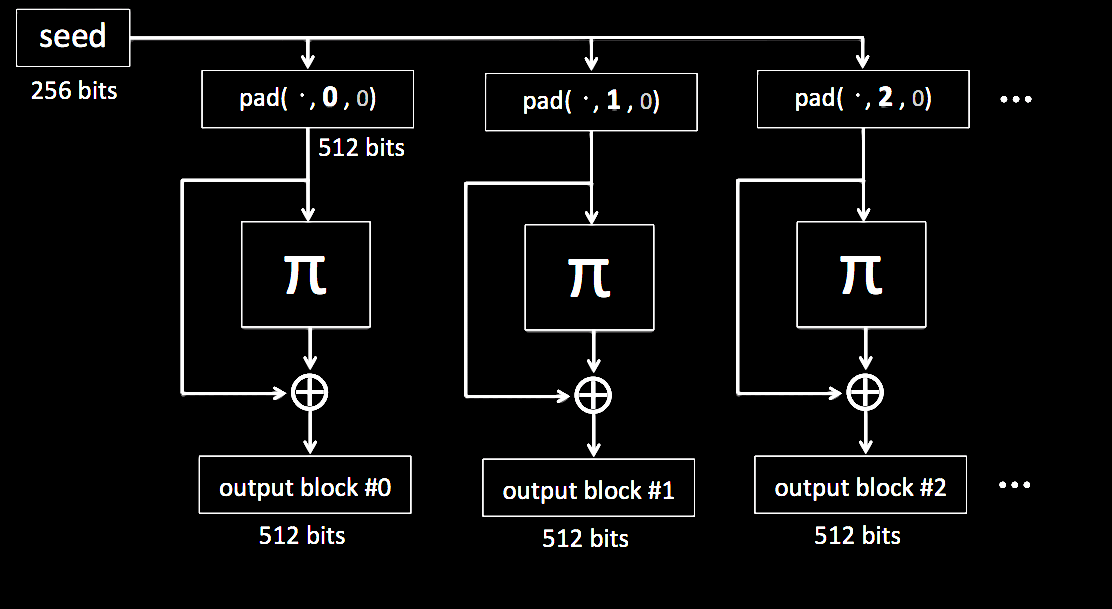
\includegraphics[width=\textwidth]{ChaCha20}
%\end{figure}
%
%Nonce -- the third parameter of $\mathsf{pad}(s, j, 0)$ is used to convert a PRG into a PRF (useful for encryption of multiple messages).
%\vfill
%\small
%{\color{gray}\textbf{picture is taken from D.Boneh, V.Shoup A Graduate Course in Applied Cryptography}} 
%\end{frame}
%
%\begin{frame}{(Somewhat) Broken PRGs}
%\LARGE
%\begin{enumerate}
%	\itemsep2em 
%	\item {\color{Orange}\textbf{linear congruential generators}} 
%	\begin{itemize}
%		\LARGE
%				\itemsep5pt  
%		\item had been used in glibc, Microsoft Visual Basic, Java
%		\item notorious for RANDU
%		\item \textbf{not cryptographically secure PRG!}
%	\end{itemize}
%
%	\item {\color{Orange}\textbf{RC4}} 
%	\begin{itemize}
%		\LARGE
%		\itemsep5pt 
%		\item proposed by R.Rivest  in 1987
%		\item used to be a part of TLS, 802.11b WEP
%		\item \textbf{not cryptographically secure PRG!}
%	\end{itemize}
%
%	\item {\color{Orange}\textbf{Linear feedback shift registers}}
%	\begin{itemize}
%			\LARGE
%			\itemsep5pt
%		\item used for protecting movies on DVD disks
%		\item weakly security  PRG (Trivium)
%	\end{itemize} 
%\end{enumerate}
%
%\end{frame}
%
%\begin{frame}{A Random Number Generator}
%	\Large
%	\begin{itemize}
%		\itemsep7pt
%		\item In practice, random bits are generated using a random number generator,  RNG
%		\item An RNG outputs a sequence of pseudorandom bits
%		\item Unlike PRG, an RNG take additional input (entropy source)
%		\item Example in Linux: $\mathsf{/dev/random}$
%		\item Entropy is usually taken from hardware (keyboard/mouse events, hardware interrupts, jitters).
%	\end{itemize}
%\end{frame}
%
%\begin{frame}{Application: Coin flipping}
%\LARGE
%Task:  throw a fair coin over without interaction 
%\begin{center}
%	\begin{tabular}{c c c c c}
%		 \multicolumn{5}{c}{$G: \{0,1\}^{\ell} \rightarrow \{0,1\}^{L}$}\\[10pt]
%		& Bob  & & Alice &  \\
%		 & \multirow{5}{*}{
\includegraphics[scale=0.20]{Bob}} & &
%		\multirow{5}{*}{
\includegraphics[scale=0.20]{Alice}} &  \\
%		&  &  & & $r \leftarrow \{0,1\}^{L}$  \\
%		&  & $\xleftarrow{r}$ & &  \\
%		Flips a coin &   & &  &  \\
%		$b \in \{0,1\}$&  & & &  \\
%		$s \in \{0,1\}^{\ell}$&  & & &  \\[15pt]
%		\multicolumn{5}{l}{$\mathsf{commit}(b, r, s)  = 
%			\begin{cases}
%			G(s), & b = 0\\
%			G(s) \oplus r, & b=1
%			\end{cases}
%			$}  \\
%		&  & $\xrightarrow{\mathsf{commit}(b, r, s)} $ & &  \\
%	\end{tabular}
%\end{center}
%
%\end{frame}

\end{document}